\chapter{\label{planificacion}Planificación}


En este apartado se establece la distribución de tiempo prevista para cada fase del trabajo, con el objetivo de presentarlo en la convocatoria de septiembre de 2026. Cada etapa incluye una estimación de duración y una fecha límite orientativa que servirá como referencia para evaluar el progreso y detectar posibles desviaciones.

Las estimaciones tienen en cuenta los riesgos identificados previamente en la matriz de riesgos, particularmente aquellos relacionados con la curva de aprendizaje en tecnologías AR/VR y la posible subestimación de la complejidad técnica. Además, se ha considerado la carga académica que supone el ABP, lo que reduce la disponibilidad efectiva de horas semanales dedicables al proyecto.

Se ha incorporado un margen de seguridad de dos semanas antes de la fecha límite oficial de entrega, previendo la aparición de imprevistos técnicos, problemas con hardware de testing o cualquier otra contingencia que pudiera surgir durante el desarrollo.

El inicio oficial del proyecto tuvo lugar el 22 de diciembre de 2025, fecha con la que se empezó a investigar herramientas técnicas y se comenzó la redacción de la memoria. Todos estos plazos se detalla en el siguiente Cuadro~\ref{tab:planificacion-temporal}. 


\begin{table}[!htb]
\centering
\caption{Planificación temporal del proyecto}
\label{tab:planificacion-temporal}
\begin{tabular}{p{8cm}cc}
\toprule
\textbf{Contenidos} & \textbf{Tiempo estimado} & \textbf{Fecha límite} \\
\midrule
Motivación, Introducción, Estudio de viabilidad & 2 semanas & 12/01/2026 \\
\addlinespace
Planificación, Estado del arte, Objetivos, Metodología & 3 semanas & 26/01/2026 \\
\addlinespace
Análisis y especificación & 3 semanas & 16/02/2026 \\
\addlinespace
Diseño & 4 semanas & 09/03/2026 \\
\addlinespace
Implementación & 10 semanas & 06/04/2026 \\
\addlinespace
Pruebas y validación, Resultados & 4 semanas & 15/06/2026 \\
\addlinespace
Conclusiones y trabajo futuro, Referencias, bibliografía y apéndices, Revisión final & 3 semanas & 06/07/2026 \\
\bottomrule
\end{tabular}
\end{table}




\chapter{\label{estado-arte}Estado del arte}

La intersección entre tecnologías inmersivas (Realidad Aumentada y Realidad Virtual) y el sector de la construcción representa un campo en constante evolución que ha experimentado un crecimiento significativo durante la última década. Para abordar adecuadamente el desarrollo de una aplicación AR/VR orientada a la visualización de proyectos arquitectónicos mediante modelos BIM, resulta imprescindible comprender el contexto tecnológico actual, las soluciones existentes en el mercado, sus fortalezas y limitaciones, así como las tendencias emergentes que están configurando el futuro del sector.

Esta sección consiste en un análisis exhaustivo del estado actual de la técnica, examinando tanto los fundamentos tecnológicos que sustentan estas aplicaciones como las propuestas comerciales y académicas más relevantes. El objetivo es adquirir una visión comprehensiva que permita identificar oportunidades de mejora, detectar funcionalidades desatendidas y establecer los requisitos técnicos necesarios para diseñar una solución que aporte valor real diferenciado.

\section{Reconstrucción volumétrica: 3D Gaussian Splatting}

El 3D Gaussian Splatting (3DGS) ha emergido recientemente como una técnica revolucionaria para la reconstrucción tridimensional y el renderizado volumétrico a partir de un conjunto de fotografías bidimensionales. A diferencia de la modelado tradicional, que intenta generar mallas poligonales cerradas y a menudo falla al interpretar superficies reflectantes, transparentes o sin textura, el 3DGS representa la escena utilizando millones de partículas matemáticas (distribuciones gaussianas 3D) que poseen atributos de posición, escala, rotación, opacidad y color armónico esférico.

Esta técnica es considerado un salto considerable respecto a métodos previos como los NeRFs (Neural Radiance Fields). Mientras que los NeRFs requieren tiempos de inferencia altísimos que imposibilitan su uso fluido\footnote{\cite{mildenhall2020nerf}}, el Gaussian Splatting permite un renderizado fotorrealista en tiempo real, alcanzando mejores tasas de fotogramas (FPS) incluso en escenas de gran complejidad geométrica.

En el contexto de la arquitectura y la construcción, esta tecnología ofrece posibilidades para el control de calidad y la auditoría de obras:

Como se puede observar en la Figura~\ref{fig:gaussian-splat}, Gaussian Splatting permite digitalizar el estado actual de una obra o apartamento con un fotorrealismo absoluto, capturando detalles milimétricos (como cableado, texturas de materiales o imperfecciones) que los escáneres láser o las mallas tradicionales suelen ignorar o deformar.

Adicionalmente, la verdadera potencia de esta tecnología en el sector constructivo reside en su superposición con los modelos teóricos. Al importar una captura de Gaussian Splatting en un entorno inmersivo junto al modelo BIM original, los profesionales pueden realizar una inspección visual directa, detectando desviaciones, errores de ejecución o interferencias estructurales antes de que supongan un sobrecoste crítico para el proyecto.


La integración de nubes de puntos volumétricas generadas mediante 3DGS como entorno de validación para modelos BIM resuelve de manera directa los conflictos existentes entre el diseño digital planificado y la realidad física construida.

\begin{figure}[!htb]
    \centering
    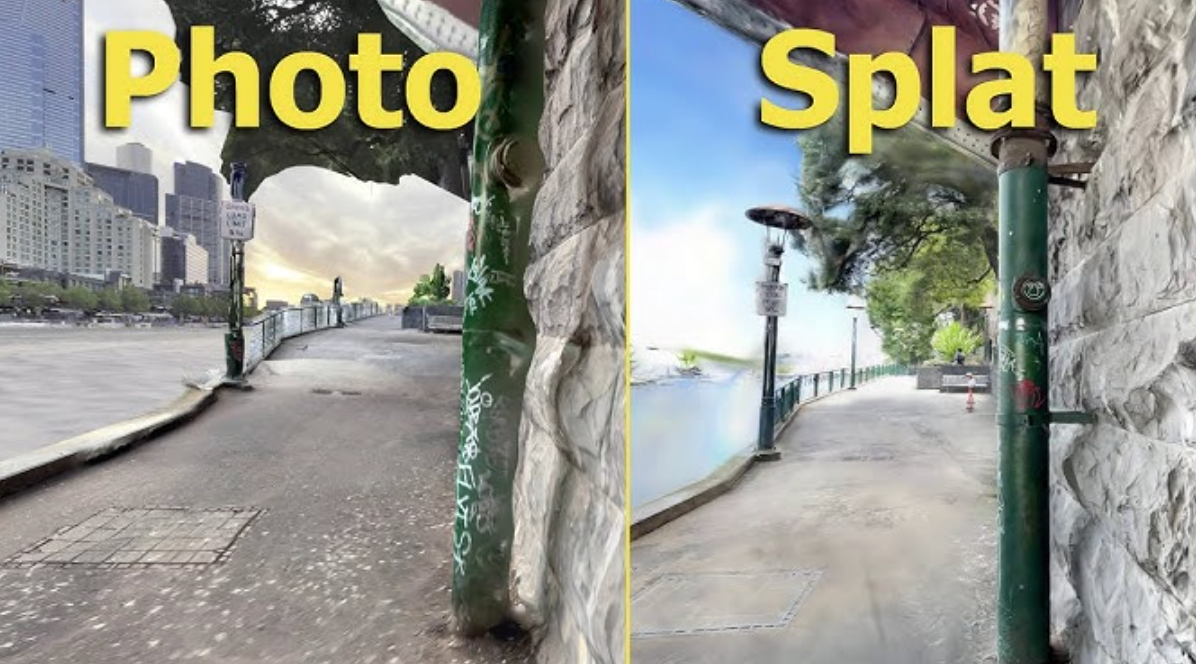
\includegraphics[width=0.8\linewidth]{include/images/figura3.1.PNG}
    \caption{Comparación Gaussian Splat con realidad}
    \label{fig:gaussian-splat}
\end{figure}


\begin{figure}[!htb]
    \centering
    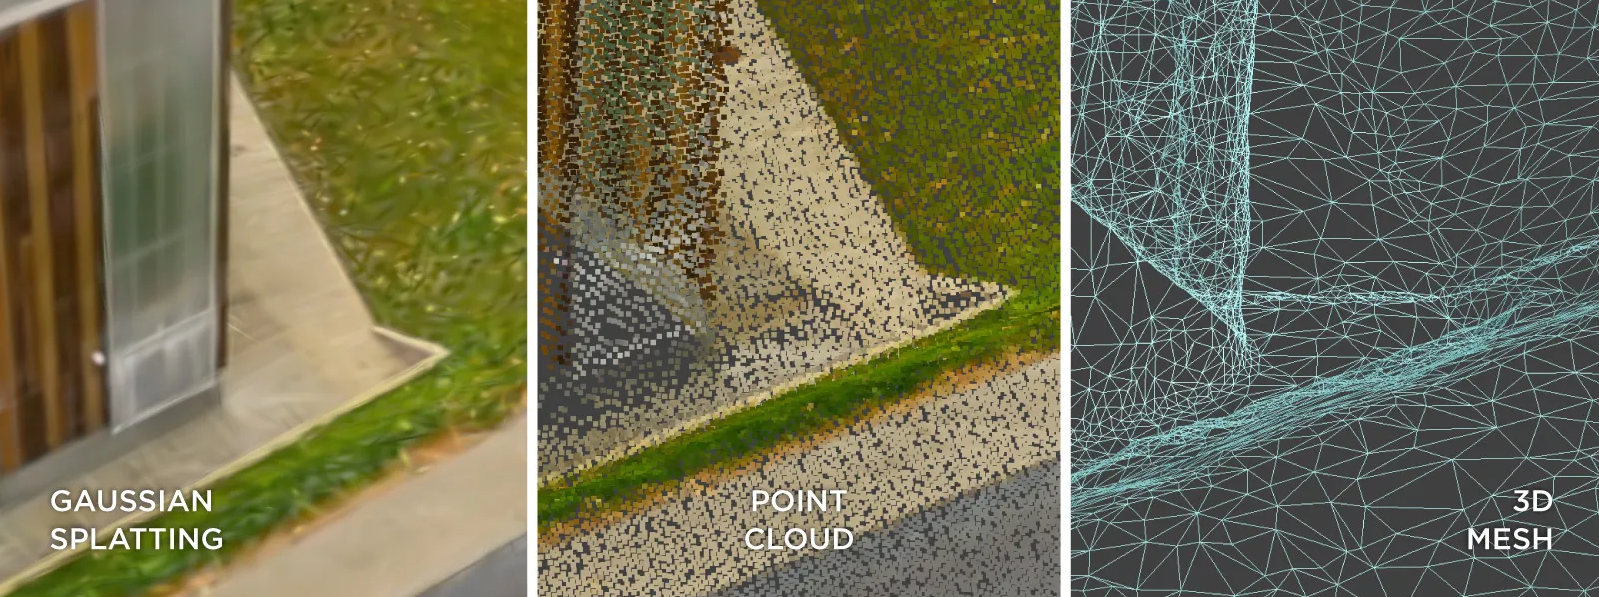
\includegraphics[width=0.8\linewidth]{include/images/gaussiancomparison.png}
    \caption{Comparación de Gaussian Splat, Point Cloud convencional y malla 3D}
    \label{fig:gaussiancomparison}
\end{figure}

\section{Metodología BIM en la construcción}
Building Information Modeling (BIM) representa un cambio paradigmático en la forma de concebir, diseñar y ejecutar proyectos de construcción\footnote{\cite{eastman2011bim}}. A diferencia de los métodos tradicionales basados en planos bidimensionales independientes, BIM propone un modelo tridimensional único y centralizado que integra información geométrica, técnica, funcional y temporal de todos los elementos constructivos.
\begin{figure}[!htb]
    \centering
    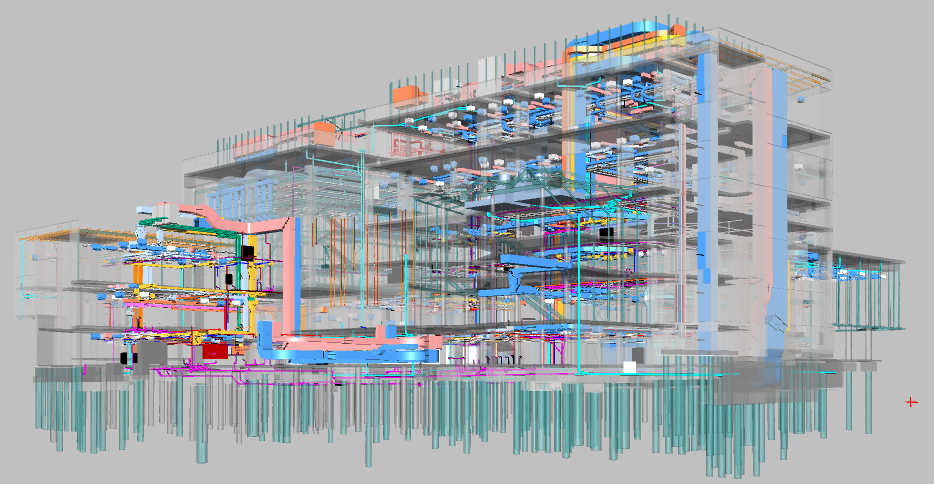
\includegraphics[width=0.8\linewidth]{include/images/BIMmodel.png}
    \caption{Edificio BIM clasificado en elementos constructivos}
    \label{fig:BIMmodel}
\end{figure}
\subsection{Evolución y adopción BIM}

La adopción de metodologías BIM ha sido progresiva pero constante. Países como Reino Unido establecieron en 2016 la obligatoriedad de utilizar BIM nivel 2 en proyectos públicos\footnote{\cite{ukcabinet2016strategy}}, mientras que la Unión Europea publicó en 2017 el manual para la introducción del BIM en contratación pública\footnote{\cite{eubim2017handbook}}. En España, aunque la implantación ha sido más gradual, la Comisión BIM creada por el Ministerio de Fomento en 2015 ha impulsado su adopción mediante recomendaciones y directrices, estableciendo diciembre de 2018 como fecha recomendada para su uso en licitaciones públicas\footnote{\cite{fomento2015comision}}.

Esta estandarización progresiva genera un ecosistema propicio para aplicaciones que consuman datos BIM, dado que cada vez más proyectos disponen de modelos digitales estructurados susceptibles de ser visualizados mediante tecnologías inmersivas.

\subsection{Formatos y estándares BIM}

La interoperabilidad constituye uno de los desafíos fundamentales del ecosistema BIM. Diferentes actores del proyecto utilizan software especializado para sus disciplinas (Revit para arquitectura, Tekla para estructuras, MEP para instalaciones), lo que genera la necesidad de formatos de intercambio que preserven la información.

IFC (Industry Foundation Classes) se ha consolidado como el estándar abierto por excelencia, desarrollado por buildingSMART International. IFC define una estructura de datos jerárquica que describe elementos constructivos (muros, forjados, ventanas), sus propiedades (materiales, dimensiones, características térmicas) y relaciones espaciales. Su carácter abierto y neutral respecto a fabricantes lo convierte en la opción preferente para garantizar interoperabilidad, aunque las implementaciones de exportación/importación en diferentes software presentan ocasionalmente inconsistencias.

Otros formatos relevantes incluyen BCF (BIM Collaboration Format) para comunicación de incidencias asociadas a elementos del modelo, COBie (Construction Operations Building Information Exchange) orientado a datos para la gestión de instalaciones, formatos propietarios como .RVT de Autodesk Revit que, aunque no abiertos, están ampliamente extendidos en la industria.

Para aplicaciones AR/VR, la conversión desde estos formatos hacia representaciones optimizadas para renderizado en tiempo real (meshes con texturas, estructuras LOD) constituye un requisito técnico que debe equilibrar fidelidad visual y rendimiento.

\subsection{Niveles de desarrollo LOD}

El concepto de Level of Development (LOD) estandariza el grado de definición geométrica y la cantidad de información asociada a los elementos BIM en diferentes fases del proyecto. La especificación más utilizada, desarrollada y estandarizada globalmente, define distintos niveles de detalle geométrico y semántico\footnote{\cite{eastman2011bim}}:
\begin{itemize}
\item LOD 100: Representación simbólica y conceptual (volúmenes aproximados)
\item LOD 200: Geometría aproximada con dimensiones, orientación y ubicación
\item LOD 300: Geometría precisa con información completa para construcción
\item LOD 400: Geometría detallada para fabricación e instalación
\item LOD 500: Modelo as-built verificado en campo
\end{itemize}

\begin{figure}[!htb]
    \centering
    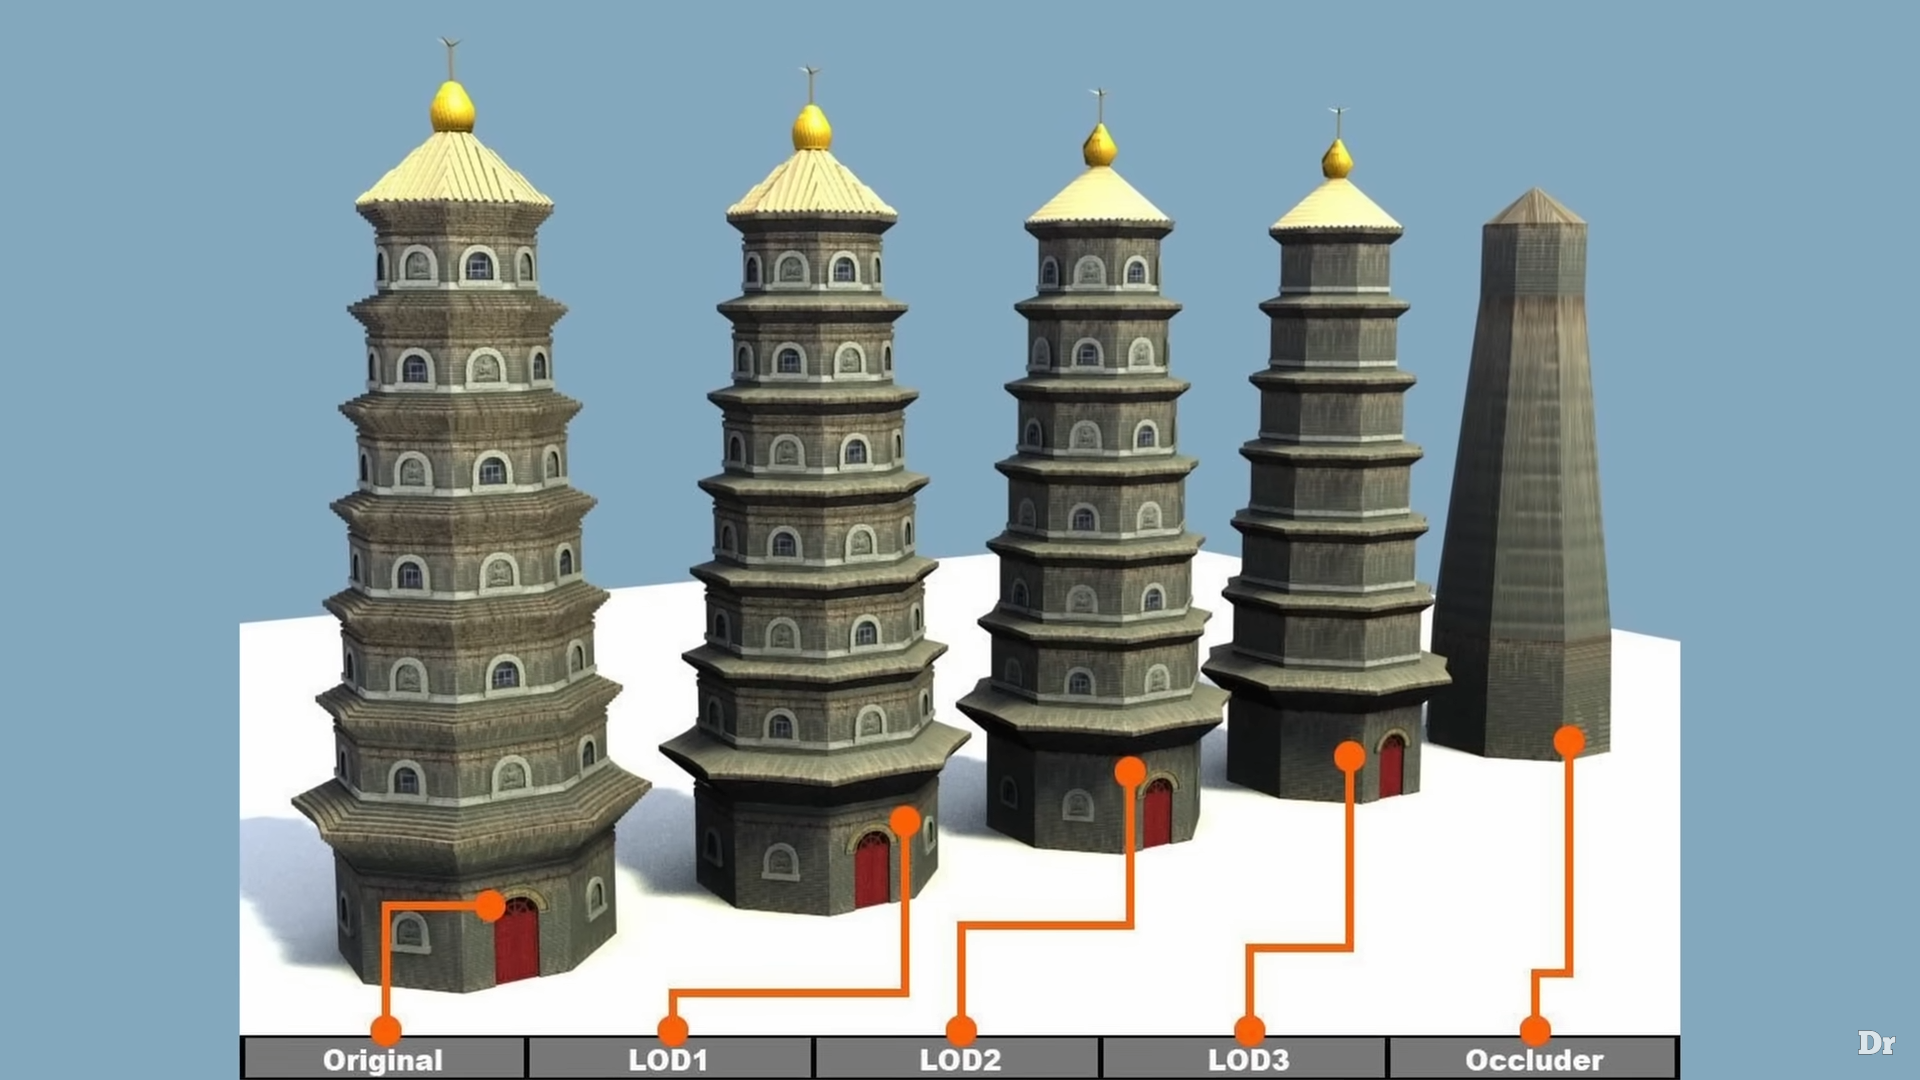
\includegraphics[width=0.8\linewidth]{include/images/lods.png}
    \caption{Ejemplos de tipos de LODs}
    \label{fig:lods}
\end{figure}
Esta gradación resulta relevante para aplicaciones AR/VR porque diferentes casos de uso requieren distintos niveles de detalle. Una presentación comercial a clientes puede funcionar perfectamente con LOD 200-300, mientras que una inspección técnica en obra podría necesitar LOD 400 para verificar encuentros constructivos complejos. Implementar sistemas de visualización que adapten automáticamente el nivel de detalle según el contexto de uso constituye un factor diferenciador importante. Como se puede ver en la siguiente Figura~\ref{fig:BIM-model}, un modelado 3D habitual coge los detalles exteriores del edificio, sin embargo, un modelo BIM analiza cada una de sus partes interiores.

\begin{figure}[!htb]
    \centering
    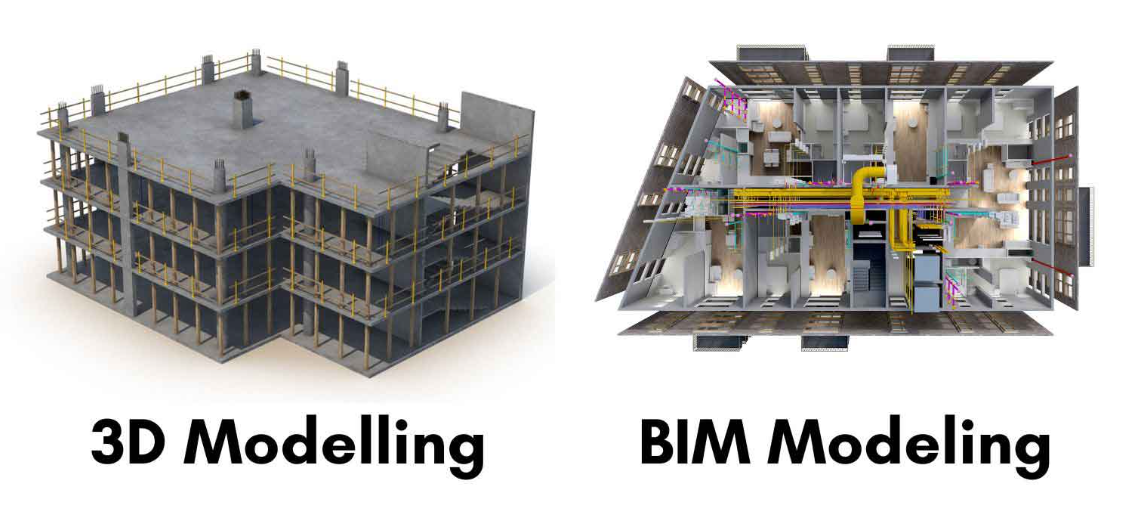
\includegraphics[width=0.8\linewidth]{include/images/figura3.2.png}
    \caption{Diferencia modelado normal con modelado BIM}
    \label{fig:BIM-model}
\end{figure}



\section{Tecnologías de Realidad Aumentada} 
En esta sección se explica toda la parte teórica relacionada con Realidad Aumentada. 
\subsection{Fundamentos técnicos de AR}


La Realidad Aumentada superpone información digital sobre la percepción del mundo real, requiriendo resolver tres desafíos técnicos fundamentales: tracking (determinar posición y orientación del dispositivo en el espacio), mapping (construir representación del entorno) y rendering (generar contenido virtual coherente con la escena real)\footnote{\cite{azuma1997survey}}.

Los sistemas modernos de AR utilizan principalmente dos enfoques de tracking:
\begin{itemize}
\item Marker-based AR: Emplea patrones visuales predefinidos (códigos QR, imágenes) que la cámara reconoce y utiliza como referencia espacial. Ofrece alta precisión en entornos controlados pero requiere preparar y mantener los marcadores físicos, lo que resulta poco práctico en obras de construcción.

\begin{figure}[!htb]
    \centering
    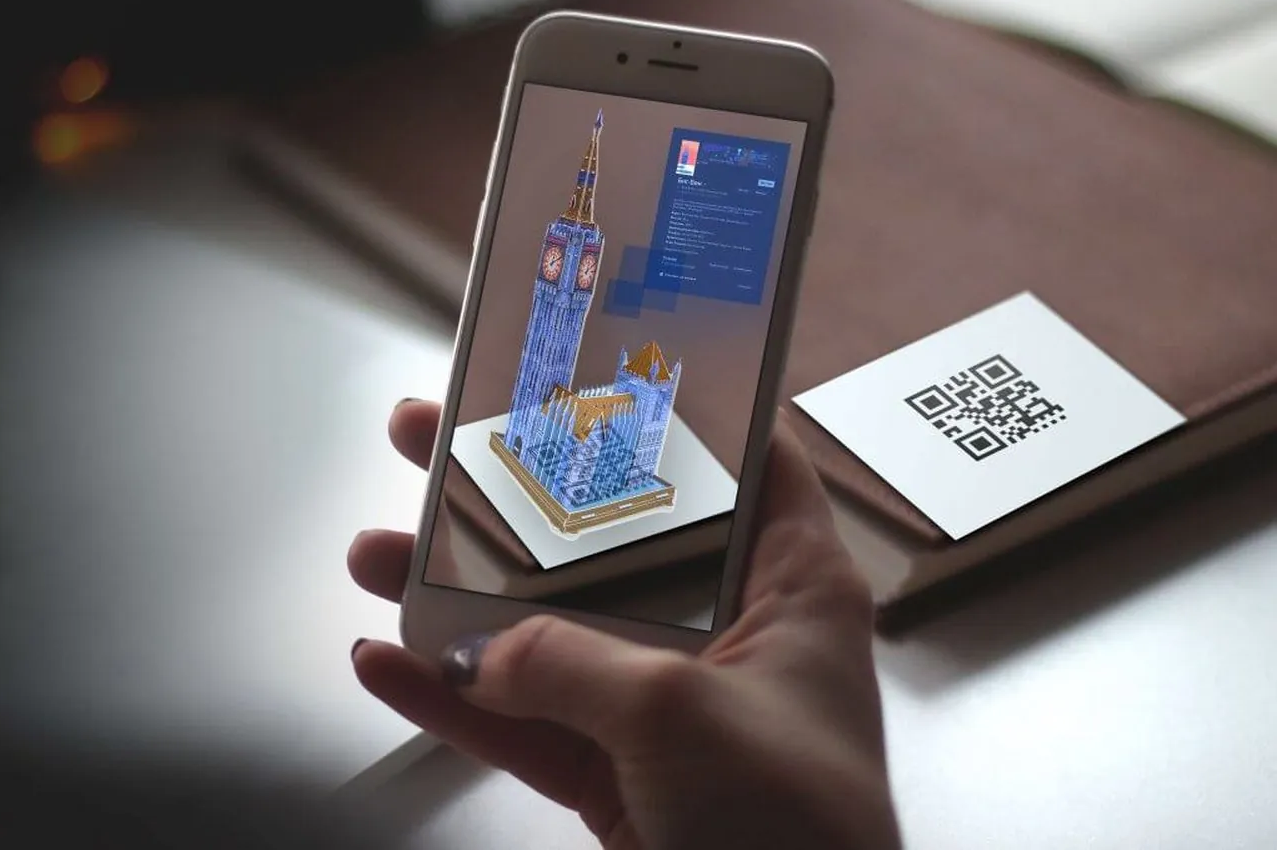
\includegraphics[width=0.8\linewidth]{include/images/markerbased.png}
    \caption{Código QR utilizado como referencia}
    \label{fig:markerbased}
\end{figure}


\item Markerless AR o SLAM: Analiza características naturales del entorno para construir un mapa espacial y posicionar el dispositivo dentro de él, lo cual conlleva desafíos de iluminación y falta de referencias en entornos de construcción\footnote{\cite{rankohi2013review}}. Este enfoque, implementado en ARCore (Google) y ARKit (Apple), permite experiencias más fluidas sin preparación previa, aunque presenta limitaciones de precisión (típicamente 5-10 cm en interiores, mayor error en exteriores).

\begin{figure}[!htb]
    \centering
    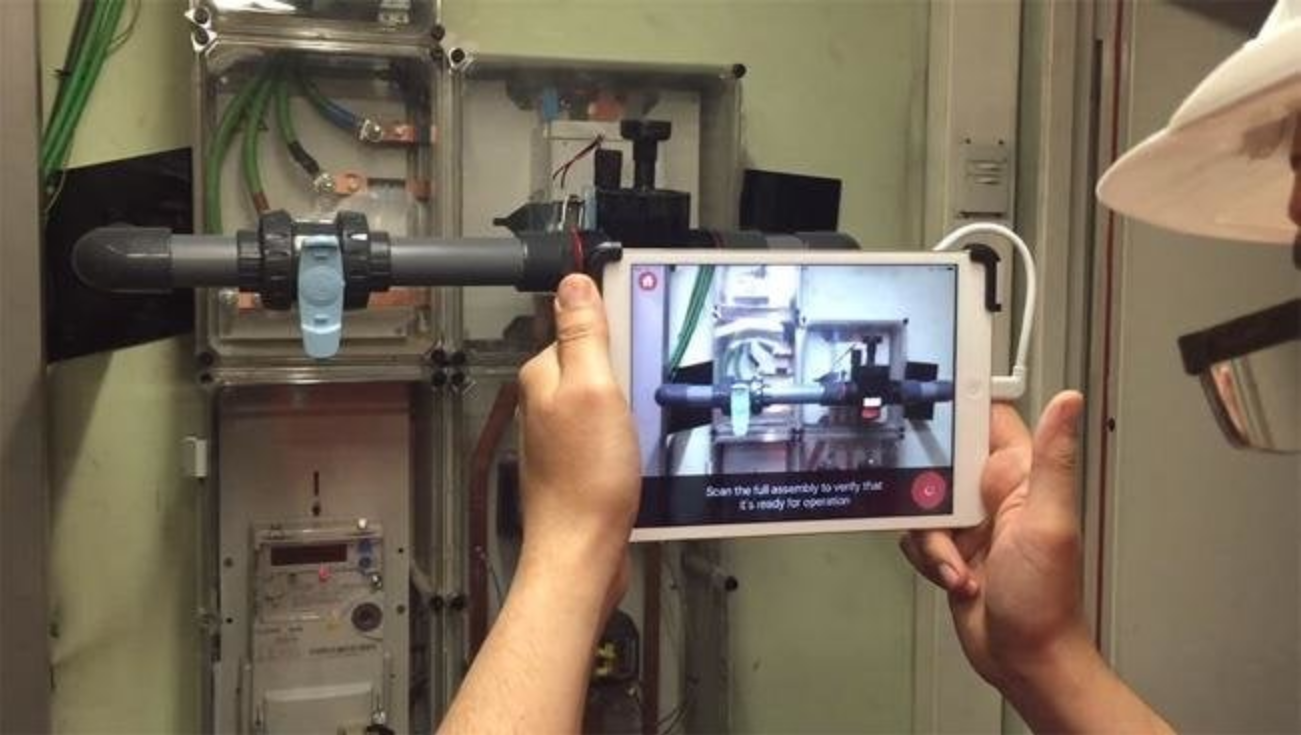
\includegraphics[width=0.8\linewidth]{include/images/markerlessar.png}
    \caption{Realidad aumentada markerless}
    \label{fig:markerlessar}
\end{figure}
\end{itemize}
Para aplicaciones en construcción, frecuentemente se necesita AR en exteriores sobre emplazamientos vacíos sin referencias visuales distintivas.

\subsection{Plataformas de desarrollo AR}

ARCore (Android) y ARKit (iOS) constituyen las plataformas dominantes para AR móvil. Ambas ofrecen APIs para detección de planos horizontales y verticales, estimación de iluminación ambiental, tracking de imágenes y rostros, y anclaje de contenido virtual. Sus capacidades son similares, aunque ARKit tradicionalmente ha mantenido ventaja en precisión de tracking gracias al control más estricto de Apple sobre el hardware.

Para aplicaciones multiplataforma, frameworks como Unity con AR Foundation o Unreal Engine con AR plugins proporcionan una capa de abstracción que permite tener la misma base desplegable en ambos ecosistemas, reduciendo significativamente el esfuerzo de desarrollo y mantenimiento.

Dispositivos especializados como Microsoft Hololens 2 o Magic Leap 2 ofrecen experiencias AR más avanzadas mediantes gafas con displays transparentes, liberando las manos del usuario y proporcionando campos de visión más amplios. Sin embargo, su elevado coste (3000-4000€ por unidad) y menor disponibilidad limitan su adopción masiva, relegándolos a casos de uso profesionales de alto valor añadido.

\begin{figure}[!htb]
    \centering
    % ---- PRIMERA IMAGEN ----
    \begin{minipage}[b]{0.48\linewidth}
        \centering
        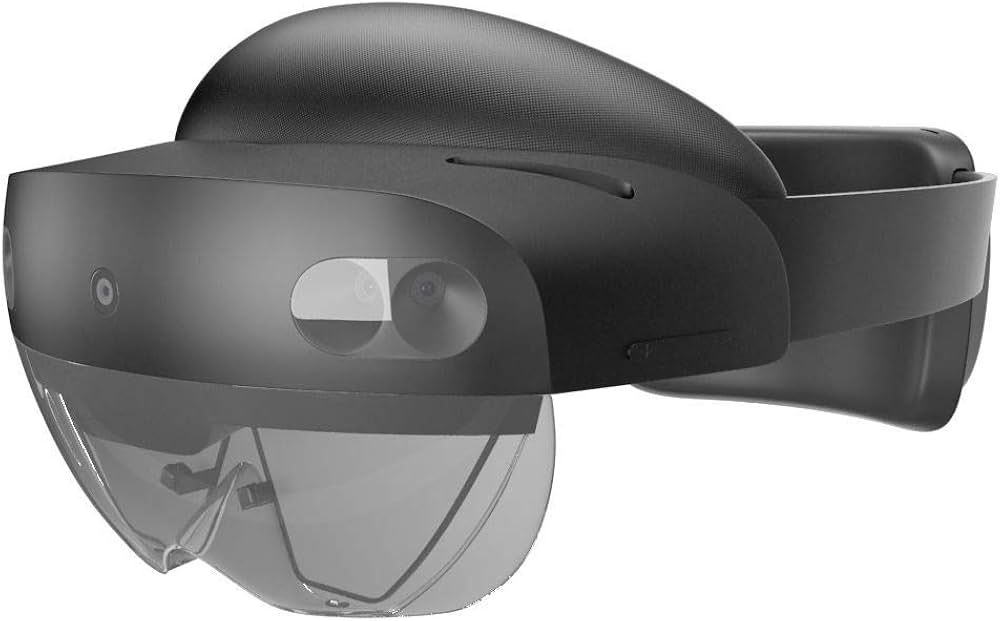
\includegraphics[width=\linewidth]{include/images/microsoftlens2.jpg}
        \caption{Gafas microsoft Lens 2}
        \label{fig:microsoftlens2}
    \end{minipage}
    \hfill
    % ---- SEGUNDA IMAGEN ----
    \begin{minipage}[b]{0.48\linewidth}
        \centering
        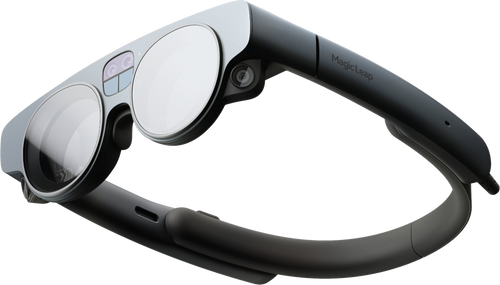
\includegraphics[width=\linewidth]{include/images/magicleap2.png}
        \caption{Gafas Magid Leap 2}
        \label{fig:magicleap2}
    \end{minipage}
\end{figure}

\subsection{Desafíos específicos de AR en construcción}

La aplicación de AR en entornos de construcción presenta particularidades que no aparecen en otros dominios:
\begin{itemize}

\item Condiciones ambientales adversas: Obras expuestas a polvo, variaciones lumínicas extremas (sol directo, sombra), lluvia o temperaturas extremas que afectan al rendimiento de cámaras y sensores.

\item Ausencia de referencias visuales: En fases tempranas, el emplazamiento puede ser un solar vacío sin características distintivas, obligando a depender de GPS con sus limitaciones de precisión\footnote{\cite{wang2013augmented}}.

\item Escala y distancias: Los proyectos arquitectónicos abarcan decenas o cientos de metros, mientras que el tracking AR optimiza para espacios interiores de pocos metros. Mantener coherencia espacial en áreas extensas requiere estrategias específicas de gestión de anclajes persistentes.

\item Complejidad geométrica: Los modelos BIM contienen millones de polígonos que superan las capacidades de renderizado en tiempo real de dispositivos móviles, necesitando técnicas agresivas de optimización (culling, LOD dinámico, instancing).
\end{itemize}
Solucionar estos desafíos constituye uno de los valores añadidos fundamentales que debe aportar una aplicación AR específicamente diseñada para construcción.


\section{Tecnologías de Realidad Virtual}
En esta sección se explica toda la parte teórica relacionada con Realidad Virtual.
\subsection{Fundamentos técnicos de VR}



La Realidad Virtual sumerge completamente al usuario en un entorno sintético mediante headsets que bloquean la visión del mundo real y presentan imágenes estereoscópicas (ligeramente diferentes para cada ojo) que generan percepción de profundidad tridimensional.

Los sistemas VR modernos ofrecen 6 grados de libertad (6DoF), tracking tanto de la orientación de la cabeza (pitch, yaw, roll) como de su posición espacial (x, y, z) permitiendo al usuario moverse naturalmente por el entorno virtual\footnote{\cite{slater2009place}}. Esto contrasta con sistemas más simples de 3DoF que solo rastrean orientación, adecuados para experiencias pasivas (visualización 360º) pero limitados para exploración activa de espacios arquitectónicos.

Los principales desafíos técnicos de VR incluyen:
\begin{itemize}
\item Latencia motora-visual: El retardo entre movimiento de cabeza y actualización de la imagen debe mantenerse por debajo de 20ms para evitar mareo. Esto exige mantener framerates elevados incluso con escenas complejas.

\item Resolución y field of view: Los displays actuales (típicamente 1832x1920 por ojo en Meta Quest 2) muestra efecto de pixelado ("screen door effect") que rompe la inmersión. Aumentar resolución compite con las demandas de framerate.

\item Ergonomía y comfort: Sesiones prolongadas pueden causar fatiga ocular, mareo (motion sickness) o incomodidad por el peso del dispositivo. El diseño de interacciones debe minimizar estos efectos mediante técnicas como teleportación en lugar de movimiento continuo con joystick en casos extremos de optimización.
\end{itemize}
\subsection{Plataformas VR y dispositivos}

El mercado VR se ha consolidado en torno a varios ecosistemas principales:
\begin{itemize}
\item Meta Quest (anteriormente Oculus) lidera en dispositivos standalone (todo incluido sin necesidad de PC), ofreciendo experiencias inalámbricas a precios asequibles (300-500€). Su capacidad de procesamiento limitada exige optimización agresiva de contenidos.

\begin{figure}[!htb]
    \centering
    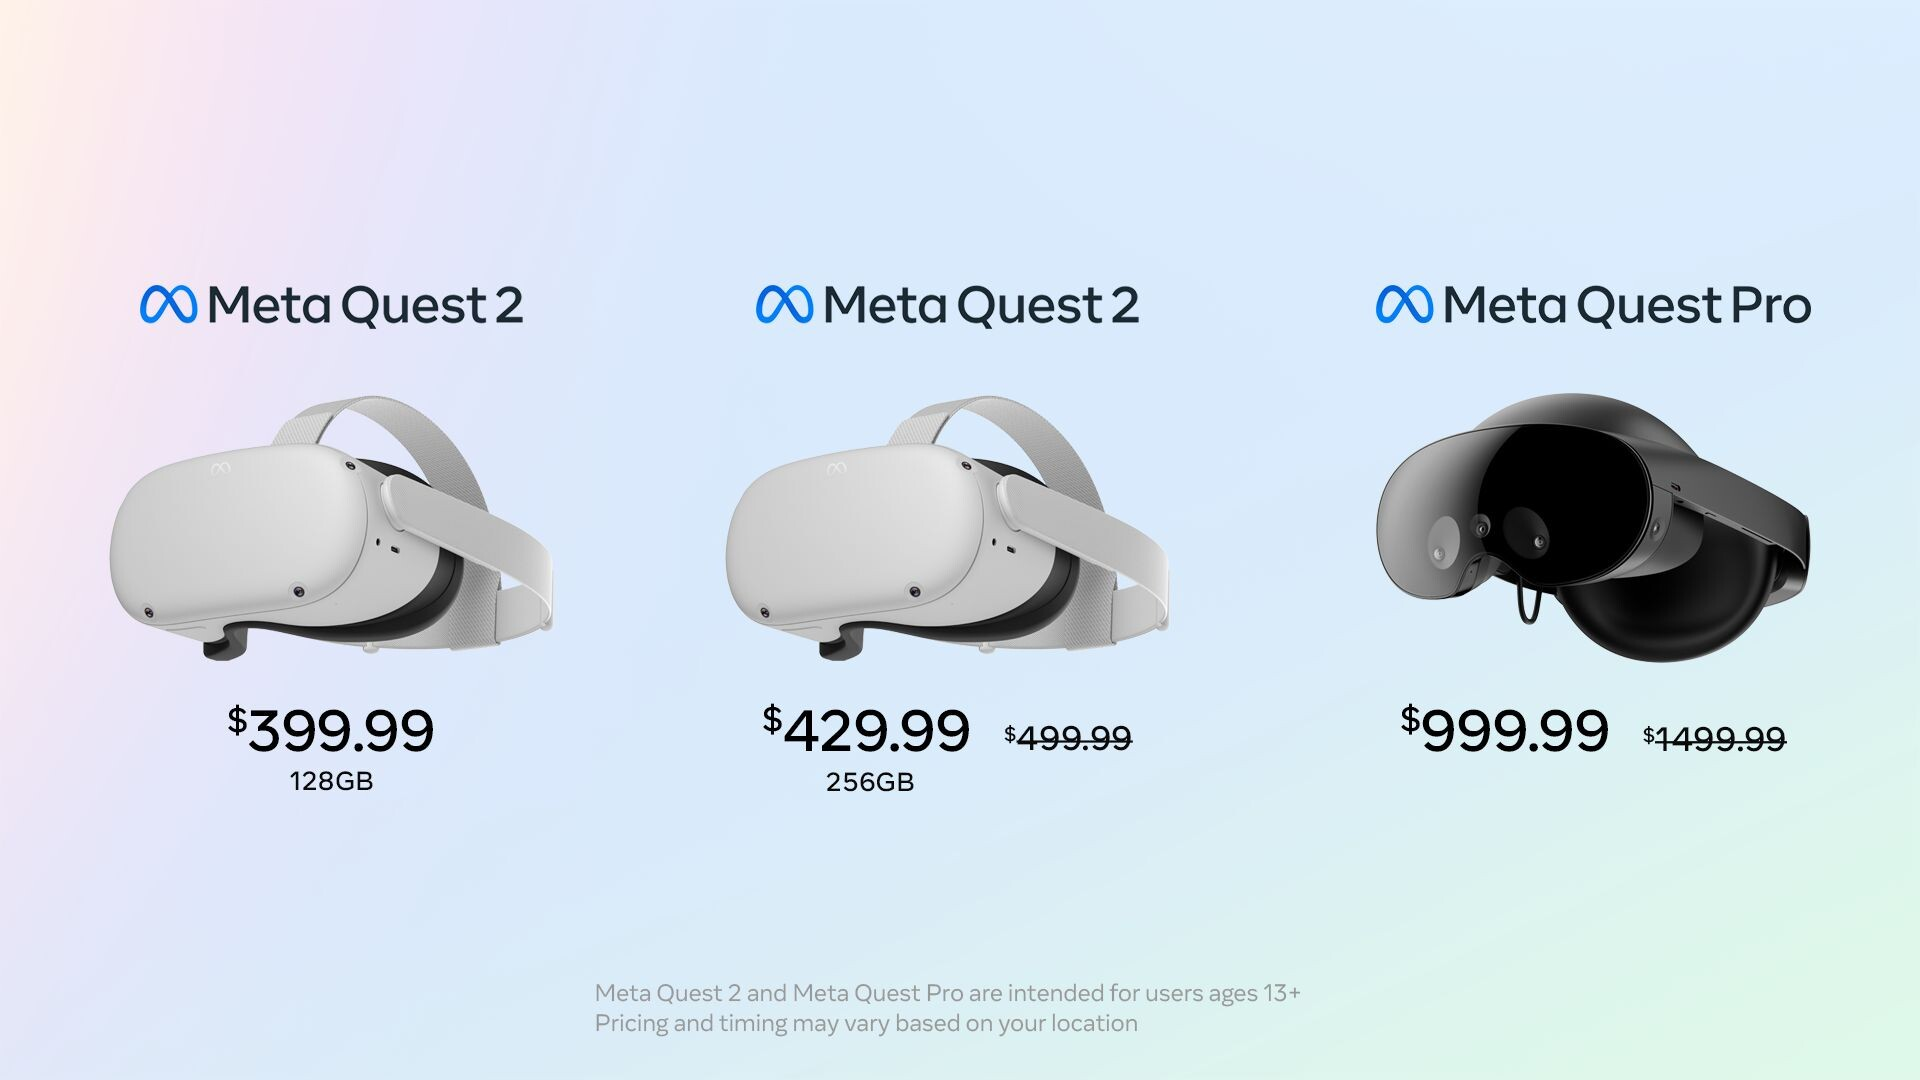
\includegraphics[width=0.8\linewidth]{include/images/questheadsets.jpg}
    \caption{Gafas de realidad virtual y precio de Meta Quest (2 y Pro)}
    \label{fig:questheadsets}
\end{figure}

\item HTC Vive/Valve Index: Representan la gama alta de VR conectada a PC, ofreciendo mayor fidelidad visual, tracking más preciso mediante estaciones base externas y controllers más avanzados, al coste de instalación más compleja y presupuestos superiores (800-1500€).

\begin{figure}[!htb]
    \centering
    % ---- PRIMERA IMAGEN ----
    \begin{minipage}[b]{0.48\linewidth}
        \centering
        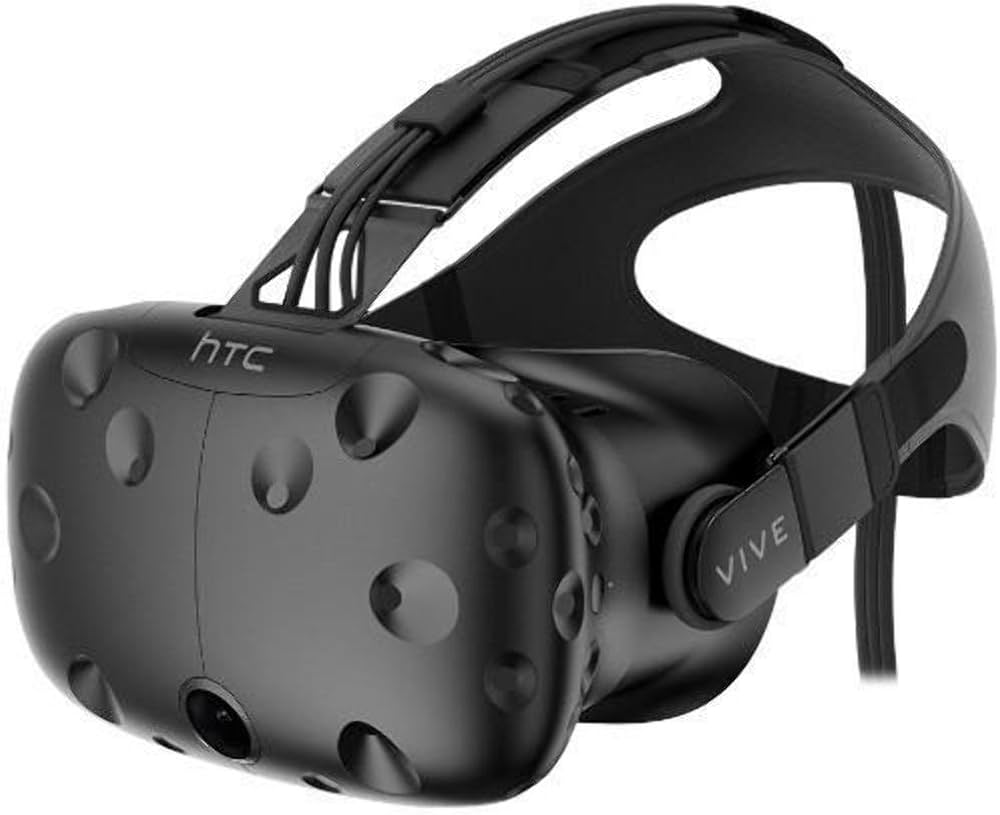
\includegraphics[width=\linewidth]{include/images/htcvive.jpg}
        \caption{Gafas HTC Vive}
        \label{fig:htcvive}
    \end{minipage}
    \hfill
    % ---- SEGUNDA IMAGEN ----
    \begin{minipage}[b]{0.48\linewidth}
        \centering
        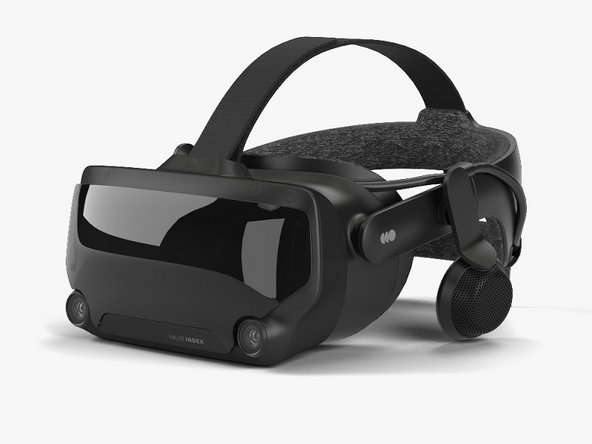
\includegraphics[width=\linewidth]{include/images/valveindex.jpg}
        \caption{Gafas Valve Index}
        \label{fig:valveindex}
    \end{minipage}
\end{figure}

\item PlayStation VR: Captura el mercado de consolas pero resulta menos relevante para aplicaciones profesionales por sus capacidades limitadas y ecosistema cerrado.

\begin{figure}[!htb]
    \centering
    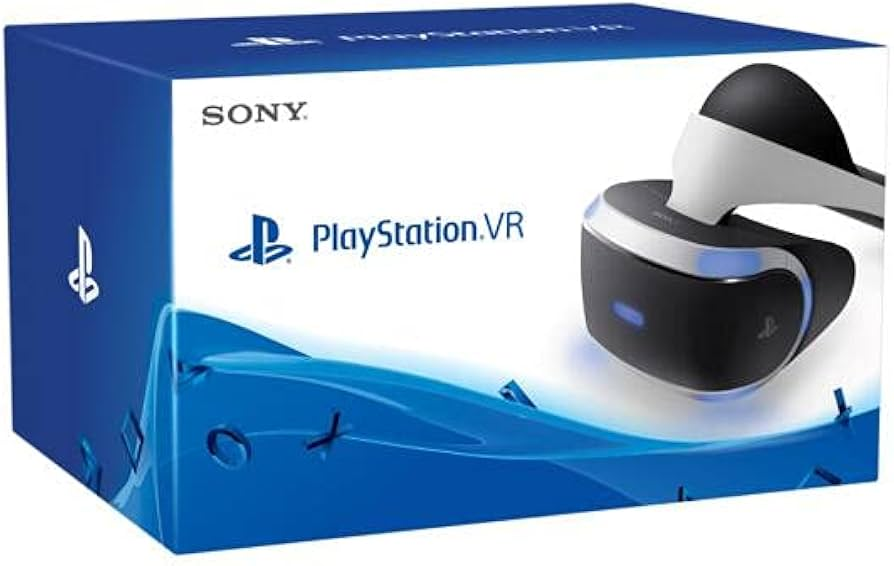
\includegraphics[width=0.8\linewidth]{include/images/psvr.jpg}
    \caption{Gafas Playstation VR}
    \label{fig:psvr}
\end{figure}


\item Pico (propiedad de ByteDance): Emerge como alternativa a Meta en mercados empresariales, ofreciendo dispositivos standalone con enfoque business y gestión de flotas.

\begin{figure}[!htb]
    \centering
    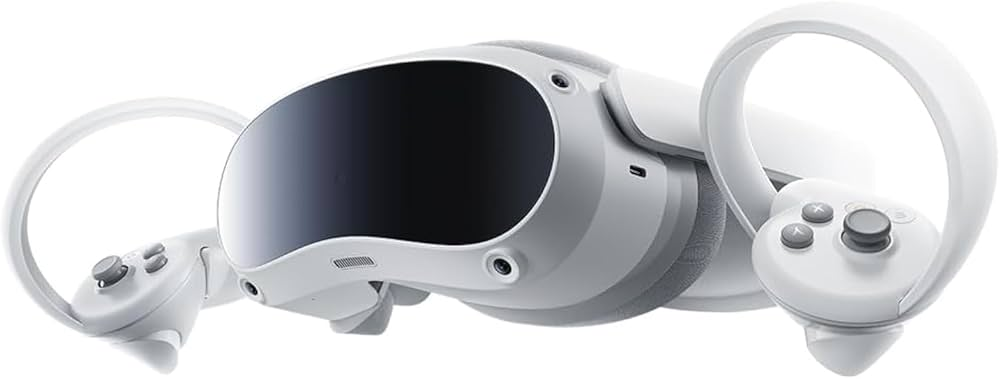
\includegraphics[width=0.8\linewidth]{include/images/pico4.jpg}
    \caption{Gafas Pico 4}
    \label{fig:pico}
\end{figure}


\end{itemize}
Para desarrollo multiplataforma, Unity y Unreal Engine vuelven a ser las opciones dominantes, soportando todos los headsets principales mediante OpenXR, el estándar abierto para VR impulsado por Khronos Group que permite desarrollar una vez y desplegar en múltiples dispositivos.

\subsection{VR aplicada a arquitectura y construcción}

VR resulta particularmente valiosa en construcción para:

- Visualización de proyectos: Permitir a clientes, inversores o autoridades experimentar espacios antes de su construcción, evaluando proporciones, iluminación natural, vistas y sensación espacial de forma imposible mediante renders estáticos o vídeos.

- Revisión de diseño: Arquitectos e ingenieros pueden detectar conflictos espaciales, evaluar ergonomía de circulaciones y validar parámetros de seguridad desde la perspectiva del usuario final\footnote{\cite{li2018critical}}.

- Formación en seguridad: Simulación de procedimientos de trabajo en altura, manejo de maquinaria o respuesta ante emergencias en entornos controlados sin riesgos reales.

- Coordinación de oficios: Visualización de instalaciones (electricidad, fontanería, climatización) en su contexto espacial real facilita detectar interferencias antes de ejecutar en obra.

Las ventajas de VR complementan las de AR: mientras AR destaca en validación in-situ sobre lo construido, VR sobresale en exploración de lo aún no construido y en contextos donde el desplazamiento físico resultaría costoso o impracticable.

\section{Análisis de soluciones existentes}
En esta sección se detallarán las aplicaciones actuales más similares a los que se pretende abarcar este proyecto.
\subsection{Fuzor: VR + BIM}

Fuzor, desarrollado por Kalloc Studios, constituye una de las propuestas más consolidadas de integración BIM-VR. Su enfoque principal es servir como visualizador inmersivo de modelos Revit (como se puede observar en la Figura~\ref{fig:Fuzor-screenshot}), estableciendo un vínculo directo (LiveLink) que sincroniza cambios en el modelo BIM con la representación VR en tiempo real\footnote{\cite{fuzor}}.

Características principales:
\begin{itemize} 
\item Integración nativa con Autodesk Revit mediante plugin
\item Soporte de múltiples headsets VR (HTC Vive, OCulus, WIndows MR)
\item Funcionalidades de clash detection (detección de colisiones) visualizadas en VR.
\item Simulación de secuencias constructivas.
\item Herramientas de medición y anotación dentro del entorno virtual.
\item Motor físico para simulación de comportamiento de objetos.
\end{itemize}
La sincronización en tiempo real con Revit representa su mayor ventaja competitiva, permitiendo a diseñadores iterar sobre el proyecto y evaluar cambios inmediatamente en VR sin exportaciones intermedias. Las capacidades de simulación 4D resultan valiosas para planificación de obra.

Sin embargo, su dependencia de Revit limita la interoperabilidad con flujos de trabajo basados en otros software BIM. No ofrece funcionalidades AR robustas para uso en campo, centrándose casi exclusivamente en VR de escritorio. El precio (licencia anual de aproximadamente 500-800€ por usuario) puede resultar prohibitivo para estudios pequeños. La curva de aprendizaje es pronunciada, requiriendo formación específica para aprovechar todas las funcionalidades.

\begin{figure}[!htb]
    \centering
    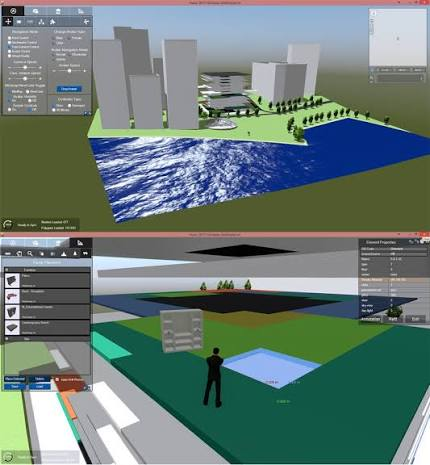
\includegraphics[width=0.7\linewidth]{include/images/figura3.3.jpg}
    \caption{Captura realizada en Fuzor}
    \label{fig:Fuzor-screenshot}
\end{figure}

\subsection{Trimble Connect: AR en construcción}

Trimble Connect forma parte del ecosistema de soluciones constructivas de Trimble, multinacional especializada en tecnologías de posicionamiento y gestión de proyectos. Como se puede apreciar en la Figura~\ref{fig:Trimble-screenshot} Su aplicación móvil AR permite visualizar modelos BIM directamente sobre el emplazamiento real mediante smartphones o tablets\footnote{\cite{trimbleconnect}}.

Caracteristicas principales:
\begin{itemize}
\item Aplicación móvil para iOS y Android
\item Importación de modelos desde múltiples fuentes BIM (Revit, SketchUp, Tekla)
\item Posicionamiento mediante GPS y alineación manual
\item Herramientas de medición y comparación modelo vs realidad
\item Sistema de issues/incidencias geolocalizadas
\item Integración con plataforma Trimble Connect para colaboración en nube
\end{itemize}
Su integración con el ecosistema Trimble (estaciones totales, escáneres láser, soluciones de topografía) proporciona ventajas significativas para empresas que ya utilizan estos equipamientos profesionales. La aplicación móvil resulta más accesible que soluciones basadas en gafas AR caras. El sistema de gestión de incidencias vinculado al modelo facilita la comunicación entre oficina técnica y obra.

Por otro lado, la precisión de posicionamiento mediante GPS resulta insuficiente para muchas tareas de inspección detallada. La interfaz, aunque funcional, no destaca por su intuitividad y requiere cierto periodo de adaptación. Las funcionalidades más avanzadas requiere suscripción a servicios Trimble Connect, generando costes recurrentes. No ofrece experiencias VR inmersivas, limitándose a AR móvil.

\begin{figure}[!htb]
    \centering
    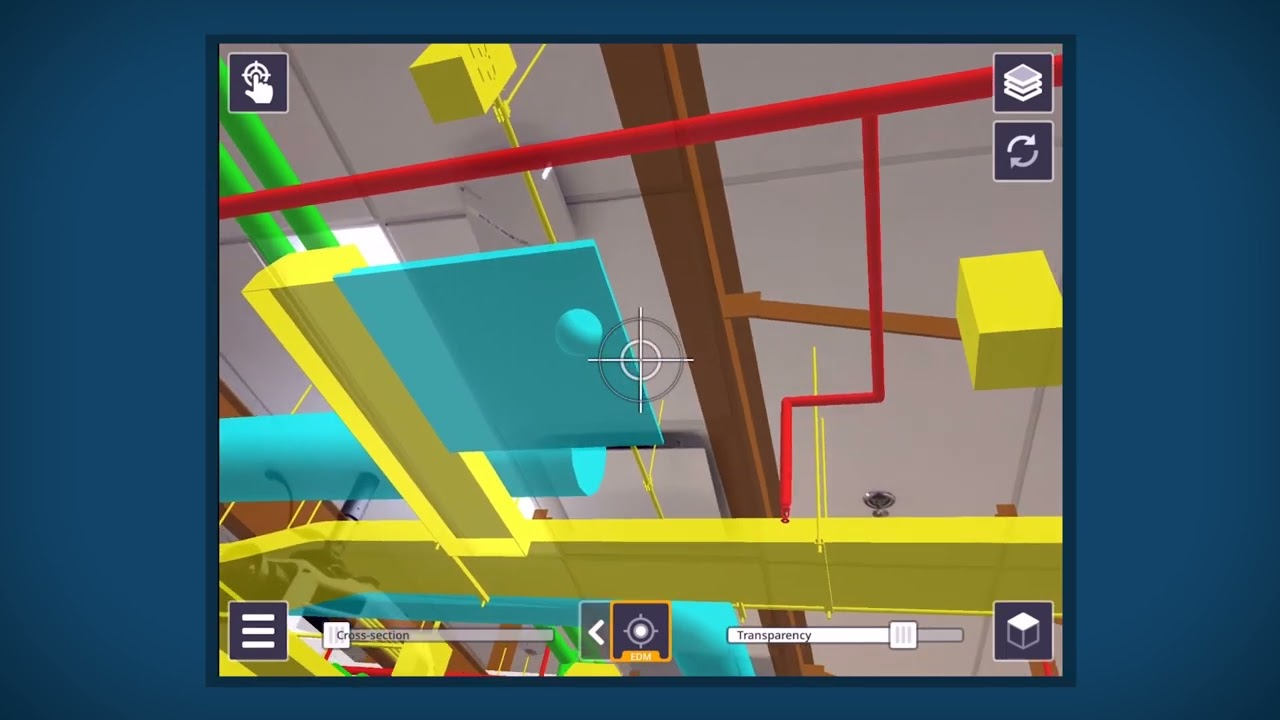
\includegraphics[width=0.7\linewidth]{include/images/figura3.4.jpg}
    \caption{Captura realizada en la aplicación móvil de Trimble}
    \label{fig:Trimble-screenshot}
\end{figure}

\subsection{IrisVR Prospect: inmersión VR multiusuario}

IrisVR Prospect (posteriormente adquirida por Techstars y actualmente parte de Resolve BIM) se especializó en crear experiencias VR de alta calidad a partir de modelos BIM, con particular énfasis en sesiones colaborativas multiusuario.

Características principales:
\begin{itemize}
\item Conversión automática de modelos BIM (Revit, Navisworks, Rhino, SketchUp) a entornos VR
\item Soporte de headsets principales (Oculus, Vive, Windows MR)
\item Modo multiusuario para reuniones virtuales dentro del modelo
\item Herramientas de medición, anotación y captura de vistas
\item Simulación de variantes de diseño (materiales, colores, configuraciones)
\item Exportación de recorridos VR para presentaciones
\end{itemize}
La calidad visual de las escenas generadas destaca sobre competidores, notándose sobre todo en materiales realistas e iluminación. Las sesiones multiusuario permiten reuniones de coordinación donde múltiples participantes (arquitectos, clientes, contratistas) exploran conjuntamente el modelo, cada uno desde su ubicación física, señalando elementos y discutiendo en tiempo real mediante audio espacializado. La simplicidad del flujo de trabajo, que consiste en importar un modelo, para después tenerlo automáticamente disponible en VR reduce barreras de entrada.

En cambio, no incluye funcionalidades AR, siendo exclusivamente una solución VR. Requiere hardware potente (PC gaming o estaciones de trabajo) para modelos complejos, limitando la portabilidad. La suscripción resulta costosa (aproximadamente 70/100€ mes por usuario), especialmente para uso ocasional. Tras la adquisición por Resolve, el desarrollo independiente de Prospect cesó, integrándose sus capacidades en la plataforma más amplia de Resolve BIM.
\subsection{Resolve BIM: plataforma integrada de coordinación}

Resolve (anteriormente conocida como BIM Track hasta 2020) representa una evolución hacia plataformas integrales que unifican coordinación BIM, gestión de incidencias y visualización inmersiva\footnote{\cite{resolvebim}}. Tras adquirir IrisVR en 2021, Resolve integró las capacidades VR de Prospect en su ecosistema más amplio de gestión de proyectos constructivos.

Características principales:
\begin{itemize} 

\item Plataforma cloud centralizada para coordinación BIM multiproyecto
\item Sistema avanzado de gestión de issues con workflows personalizables
\item Visualización 3D web (sin necesidad de software específico) de modelos BIM
\item Módulo VR heredado de IrisVR Prospect para inmersión y reuniones virtuales, mostrado en la Figura~\ref{fig:ResolveBIM-screenshot}
\item Clash detection (detección de colisiones) con priorización inteligente
\item Integración con Revit, Navisworks, Solibri y otros software BIM mediante plugins
\item Sistema de reportes y analíticas sobre estado del proyecto
\item Aplicación móvil para consulta y resolución de incidencias en campo
\end{itemize}
La principal ventaja de Resolve radica en su enfoque holístico, no es simplemente una herramienta de visualización AR/VR, sino una plataforma completa de gestión que incluye capacidades inmersivas como un componente más del flujo de trabajo. Esto facilita la trazabilidad completa desde la detección de un conflicto en VR hasta su asignación, seguimiento y verificación de resolución. El sistema de issues es particularmente robusto, con clasificación por disciplinas, estados, responsables y prioridades, generando dashboards ejecutivos que proporcionan visibilidad del estado global del proyecto.

La visualización web 3D representa otra fortaleza significativa, cualquier stakeholder con navegador puede explorar el modelo sin instalar software especializado ni tener conocimientos técnicos avanzados. Esto democratiza el acceso a la información del proyecto, facilitando la colaboración con clientes, autoridades regulatorias o subcontratistas que no manejan software BIM.

El módulo VR, aunque derivado de IrisVR Prospect, se integra perfectamente con el resto de la plataforma, las incidencias detectadas durante sesiones VR se crean automáticamente en el sistema de gestión, asignan a responsables y rastrean hasta su cierre, cerrando el ciclo de coordinación.

A pesar de sus virtudes, Resolve presenta limitaciones importantes para ciertos casos de uso. No ofrece funcionalidades AR móvil para inspección en obra, centrándose en coordinación de oficina técnica. La experiencia VR, aunque integrada, no ha evolucionado significativamente desde la adquisición de IrisVR, manteniendo las mismas limitaciones de requerir PC potente y headset dedicado.

El modelo de negocio basado en suscripción por proyecto (no solo por usuario) puede resultar costoso para estudios que manejan múltiples proyectos simultáneamente pequeños. La complejidad de la plataforma, si bien justificada por su amplitud funcional, genera curvas de aprendizaje pronunciadas que requieren inversión en formación para aprovechamiento óptimo.

Otra limitación destacable es la dependencia de conectividad, trabajar sin conexión a internet resulta problemático, lo cual puede ser restrictivo en obras donde la conectividad es inestable o inexistente. Aunque existe aplicación móvil, sus capacidades están limitadas principalmente a consulta y anotación básica, sin permitir acceder a todas las funcionalidades disponibles en la versión desktop.

Finalmente, la integración VR heredada de IrisVR no aprovecha las tendencias más recientes como headsets standalone (requiere conexión a PC), realidad mixta o funcionalidades colaborativas AR, manteniéndose como una solución VR "tradicional" en un mercado que evoluciona rápidamente hacia experiencias más versátiles.

\begin{figure}[!htb]
    \centering
    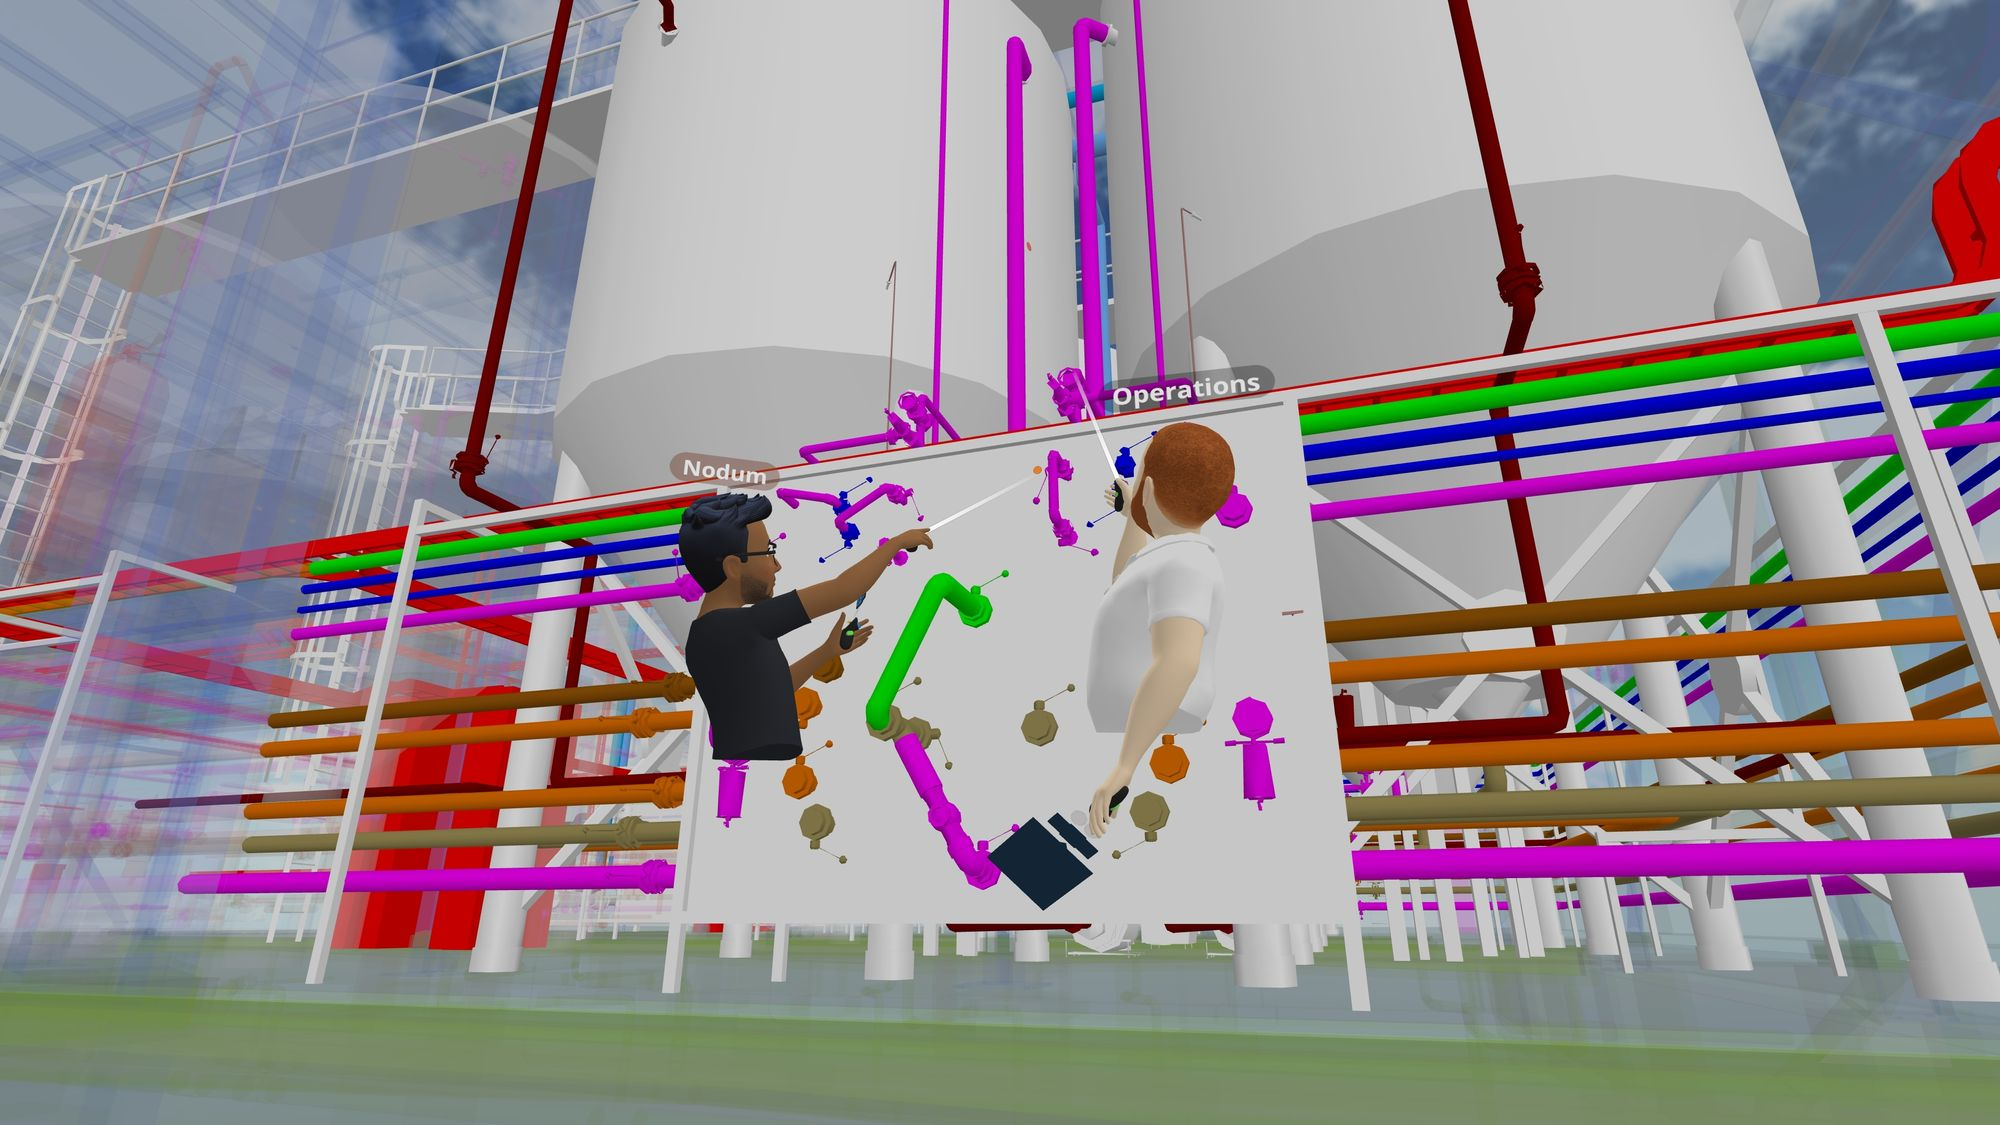
\includegraphics[width=0.8\linewidth]{include/images/figura3.5.jpg}
    \caption{Captura realizada en ResolveBIM}
    \label{fig:ResolveBIM-screenshot}
\end{figure}




\subsection{Análisis comparativo}

\begin{table}[!htb]
\centering
\caption{Análisis comparativo de soluciones existentes}
\label{tab:comparativa-soluciones}
\small
\begin{tabular}{p{4cm}cccc}
\toprule
\textbf{Característica} & \textbf{Fuzor} & \textbf{Trimble} & \textbf{IrisVR} & \textbf{Resolve} \\
\midrule
Soporte AR móvil & No & Sí & No & No \\
\addlinespace
Soporte VR & Sí (excelente) & No & Sí (excelente) & Sí (bueno) \\
\addlinespace
Integración Revit & Directa & Importación & Importación & Plugin \\
\addlinespace
Interoperabilidad BIM & Limitada & Amplia & Amplia & Amplia \\
\addlinespace
Colaboración multiusuario & Limitada & Sí (cloud) & Sí (VR) & Sí (cloud + VR) \\
\addlinespace
Gestión de issues & Básica & Buena & Básica & Excelente \\
\addlinespace
Uso en campo/obra & No & Sí (móvil) & No & Limitado \\
\addlinespace
Visualización web & No & Sí (básica) & No & Sí (avanzada) \\
\addlinespace
Curva aprendizaje & Pronunciada & Media & Suave & Pronunciada \\
\addlinespace
Coste & Alto & Medio & Alto & Alto \\
\addlinespace
Precisión posicionamiento & N/A & Media (GPS) & N/A & N/A \\
\addlinespace
Enfoque principal & VR & AR campo & VR & Gestión integral \\
\bottomrule
\end{tabular}
\end{table}


Ninguna de las soluciones analizadas en el Cuadro~\ref{tab:comparativa-soluciones} cubre completamente el espectro de necesidades identificado. Fuzor e IrisVR destacan en VR pero no ofrecen AR móvil para uso en obra. Trimble Connect proporciona AR en campo pero carece de experiencias VR inmersivas. Resolve BIM ofrece la plataforma de gestión más completa e integra VR, pero no incluye capacidades AR para inspección en campo y presenta barreras de entrada significativas en coste y complejidad.

Todas las soluciones presentan limitaciones en accesibilidad (coste, curva de aprendizaje o requisitos hardware) que restringen su adopción por pequeños estudios o profesionales independientes, configurando un espacio de oportunidad para propuestas más equilibradas que integren AR y VR manteniendo usabilidad y costes controlados.

\section{Tendencias emergentes y oportunidades}
En esta sección se explicará algunas técnicas de desarrollo para optimizar el uso de las técnologías inmersivas.
\subsection{Realidad mixta (MR) y pass-through AR}

Dispositivos recientes como Meta Quest Pro o Apple Vision Pro difuminan la frontera entre AR y VR mediante pass-through de alta calidad: cámaras frontales capturan el entorno real y lo presentan en los displays del headset, sobre el cual se superpone contenido virtual\footnote{\cite{milgram1994taxonomy}}. Esto permite transiciones fluidas entre inmersión total (VR) y el entorno real (AR) sin cambiar de dispositivo.

Esta convergencia tecnológica abre oportunidades para aplicaciones híbridas que combinen exploración VR de modelos BIM con validación AR sobre lo construido, todo dentro de un mismo flujo de trabajo y dispositivo.
\subsection{Inteligencia artificial aplicada a BIM}

El procesamiento de modelos BIM mediante técnicas de machine learning permite automatizar tareas tediosas como:\footnote{\cite{pan2021artificial}} 
\begin{itemize}
    
\item Simplificación inteligente de geometrías preservando características relevantes
\item Detección automática de conflictos más allá de colisiones geométricas (normativa, constructibilidad)
\item Generación de rutas óptimas de recorrido virtual según criterios personalizables
\item Clasificación automática de elementos para aplicar LODs diferenciados
\end{itemize}
Integrar estas capacidades en una aplicación AR/VR mejoraría significativamente la experiencia de usuario reduciendo intervención manual.

\subsection{Gemelos digitales (Digital Twins)}

El concepto de gemelos digitales extiende BIM más allá de la fase de diseño y construcción, consisten en mantener un modelo digital actualizado durante toda la vida útil del edificio, con todos sus detalles. Sensores IoT (temperatura, humedad, ocupación, consumo energético) alimentan el modelo con datos en tiempo real, dotando de semántica al espacio tridimensional\footnote{\cite{boje2020towards}}. En la Figura~\ref{fig:Gemelos-digitales} se puede apreciar y entender mejor el concepto, consiste en una réplica exacta no física.

Visualizar estos digital twins mediante AR/VR permitiría a gestores de instalaciones ver información operativa contextualizada espacialmente: "esta sala está a 26°C según el sensor, superando el umbral configurado". Esta convergencia BIM-IoT-AR representa una tendencia de crecimiento significativo en la gestión de las instalaciones.


\begin{figure}[!htb]
    \centering
    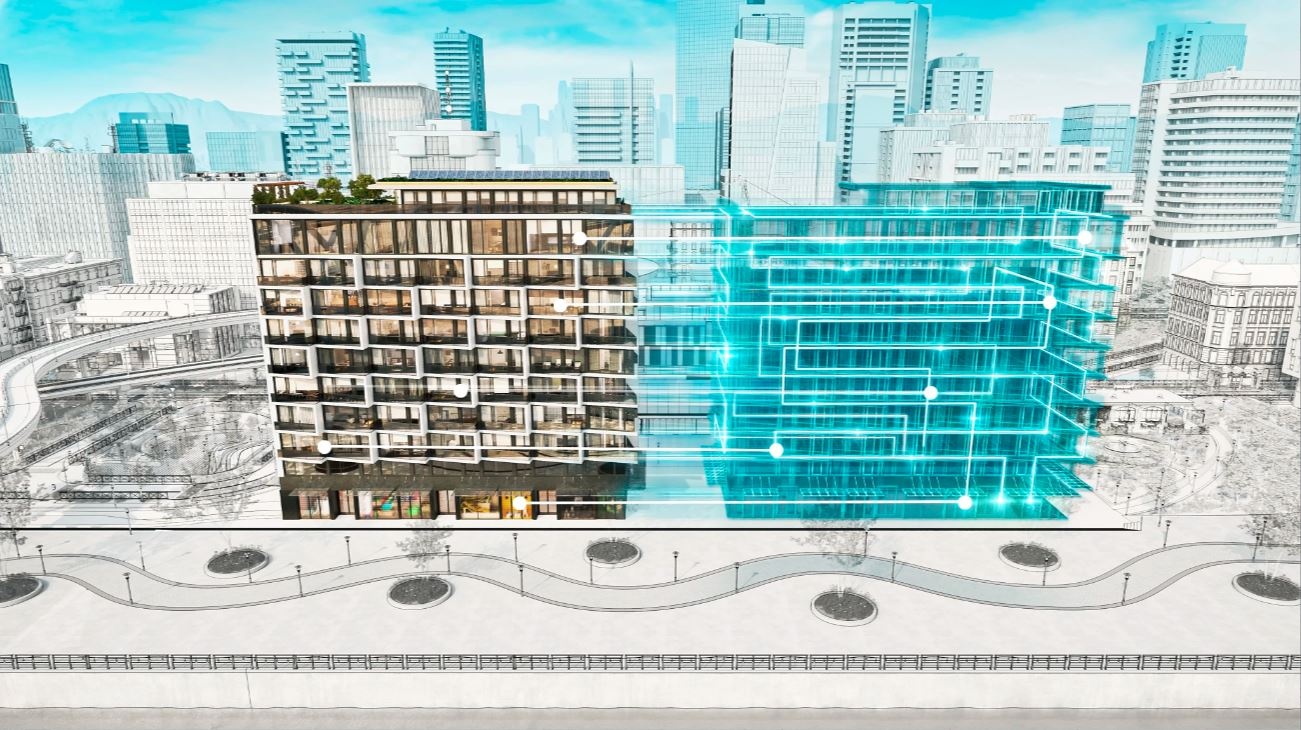
\includegraphics[width=0.8\linewidth]{include/images/figura3.6.jpg}
    \caption{Gemelos digitales}
    \label{fig:Gemelos-digitales}
\end{figure}

\subsection{5G y edge computing}

La latencia reducida y ancho de banda aumentado de redes 5G habilita arquitecturas de renderizado en la nube donde el procesamiento gráfico pesado se ejecuta en servidores y solo se transmite el vídeo resultante al dispositivo móvil. Esto permitiría visualizar modelos BIM complejos en smartphones de gama media, democratizando el acceso a experiencias de alta calidad sin depender de hardware costoso.

Combinado con edge computing (procesamiento cerca del usuario), se podrían ofrecer experiencias colaborativas multiusuario en tiempo real sin las limitaciones actuales de sincronización.

\section{Conclusiones del estado del arte}

El análisis realizado revela un panorama tecnológico maduro en sus fundamentos (AR, VR, BIM) pero que todavía está fragmentado en su aplicación práctica al sector construcción. Las soluciones comerciales existentes destacan en aspectos específicos pero ninguna integra de forma óptima AR móvil para campo, VR inmersiva para diseño y presentación, e interoperabilidad BIM amplia, manteniendo simultáneamente accesibilidad (coste, usabilidad) para pequeños y medianos profesionales.

Esta situación configura un espacio de oportunidad claro para una propuesta que:
\begin{itemize}

\item Priorice interoperabilidad mediante soporte robusto de IFC y otros formatos abiertos.
\item Ofrezca tanto experiencias AR (móvil, accesible) como VR (inmersiva, impactante) con flujo de trabajo unificado.
\item Implemente técnicas avanzadas de optimización para manejar modelos BIM complejos en hardware modesto.
\item Diseñe interfaces específicamente para usuarios del sector (arquitectos, ingenieros, constructores) minimizando curva de aprendizaje.
\item Adopte modelo de negocio accesible (freemium con funcionalidades core gratuitas) que reduzca barreras de entrada.
\end{itemize}

Los fundamentos tecnológicos están disponibles y maduros. Las metodologías BIM están consolidándose como estándar industrial. Los dispositivos AR/VR son cada vez más accesibles y potentes. El conocimiento adquirido sobre el estado del arte proporciona la base necesaria para diseñar una solución que aprenda de los aciertos y evite las limitaciones de propuestas anteriores, aportando valor diferencial real al sector de la construcción.


















\chapter{\label{objetivos}Objetivos}

En este apartado se establecen las metas y finalidades que guiarán el desarrollo del proyecto, definiendo su alcance y propósito. Se presenta primero el objetivo general, seguido de una serie de objetivos específicos que delimitan las diferentes áreas de trabajo necesarias para alcanzar el resultado esperado.

El objetivo principal de este Trabajo de Fin de Grado es diseñar, desarrollar e implementar una aplicación multiplataforma que integre tecnologías de Realidad Aumentada y Realidad Virtual para la visualización, validación e inspección de proyectos arquitectónicos mediante modelos BIM, facilitando la comunicación entre profesionales del sector construcción, mejorando la detección temprana de errores y democratizando el acceso a tecnologías inmersivas en el ámbito de la edificación. Los objetivos específicos son los siguientes:

\begin{itemize}
\item Investigar y dominar los fundamentos técnicos de las tecnologías AR/VR, adquiriendo competencias en frameworks de desarrollo (Unity con AR Foundation), sistemas de tracking espacial y optimización de renderizado en tiempo real para dispositivos móviles/gafas de Realidad Virtual.
\item Comprender en profundidad la metodología BIM y los estándares de intercambio de información en el sector construcción, familiarizándose con el formato IFC, niveles de desarrollo LOD y flujos de trabajo típicos en estudios de arquitectura e ingeniería.
\item Desarrollar un sistema robusto de importación y optimización de modelos BIM que permita convertir archivos IFC en representaciones 3D optimizadas para visualización AR/VR en dispositivos con capacidades de procesamiento limitadas.
\item Implementar funcionalidades AR móviles que permitan superponer modelos BIM sobre emplazamientos reales, utilizando posicionamiento GPS combinado con alineación manual para garantizar precisión suficiente en contextos de obra.
\item Implementar experiencias VR inmersivas que faciliten la exploración virtual de proyectos arquitectónicos antes de su construcción, proporcionando herramientas de navegación intuitivas y sistemas de interacción naturales.
\item Incorporar herramientas de anotación y reporte que permitan a los usuarios marcar discrepancias, añadir comentarios y capturar evidencias fotográficas directamente sobre los modelos visualizados, generando documentación estructurada útil para coordinación de equipos.
\item Diseñar interfaces de usuario intuitivas y específicas para profesionales del sector construcción, minimizando la curva de aprendizaje y priorizando la usabilidad en condiciones reales de trabajo (campo, obra, reuniones con clientes).
\item Garantizar la interoperabilidad mediante estándares abiertos, evitando dependencias con software propietario específico y facilitando la integración en flujos de trabajo heterogéneos donde coexisten diferentes herramientas BIM.
\item Aplicar buenas prácticas de ingeniería del software, generando código modular, bien documentado y mantenible, que facilite futuras extensiones o adaptaciones del sistema por parte de otros desarrolladores.

\end{itemize}
La consecución de estos objetivos permitirá obtener un prototipo funcional que demuestre la viabilidad técnica y el valor potencial de integrar tecnologías AR/VR con metodologías BIM en el sector de la construcción, contribuyendo tanto al aprendizaje personal como al avance del conocimiento en este campo emergente.



